実験2では, 認証機構の追加がネットワークにどれだけの負荷を与えるのかを
調査するための実験を行った. 具体的には, 
不正ノードの存在しない環境で, 250回シミュレーションを行い, 
遅延時間とオーバーヘッドサイズを調べた. 
実験2の主なシミレーションパラメータは表\ref{tab:exp2-params}に示す通りである. 
\begin{longtable}{cc}
  \caption{実験2のシミュレーションパラメータ}
  \label{tab:exp2-params}
  \endfirsthead
  \hline
  シミュレーション時間 & 300[s] \\
  ノード数 & 74 \\
  送受信ノードのペア数 & 1 \\ 
  不正ノード & なし \\ \hline
\end{longtable}
\vspace{1em}
\indent 実験結果を図\ref{fig:exp2_delay}, 図\ref{fig:exp2_overhead}に示す. \\[-2.5em]
\begin{figure}
  \centering
  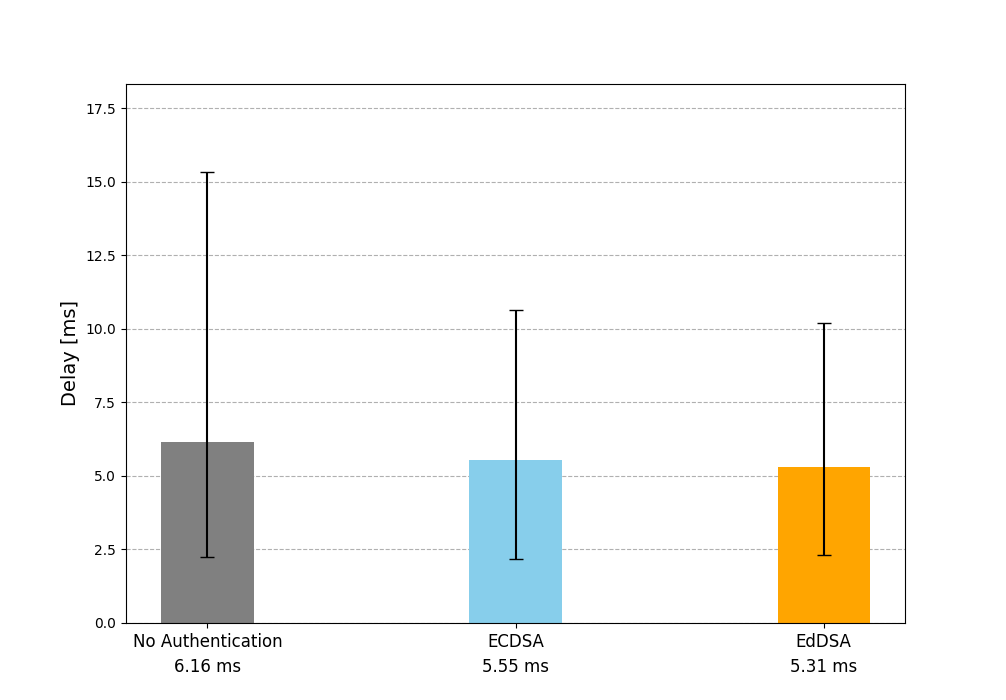
\includegraphics[width=1\textwidth]{figures/exp2_delay.png}
  \caption{不正ノードが存在しない環境での遅延時間}
  \label{fig:exp2_delay}
\end{figure}
\begin{figure}
  \centering
  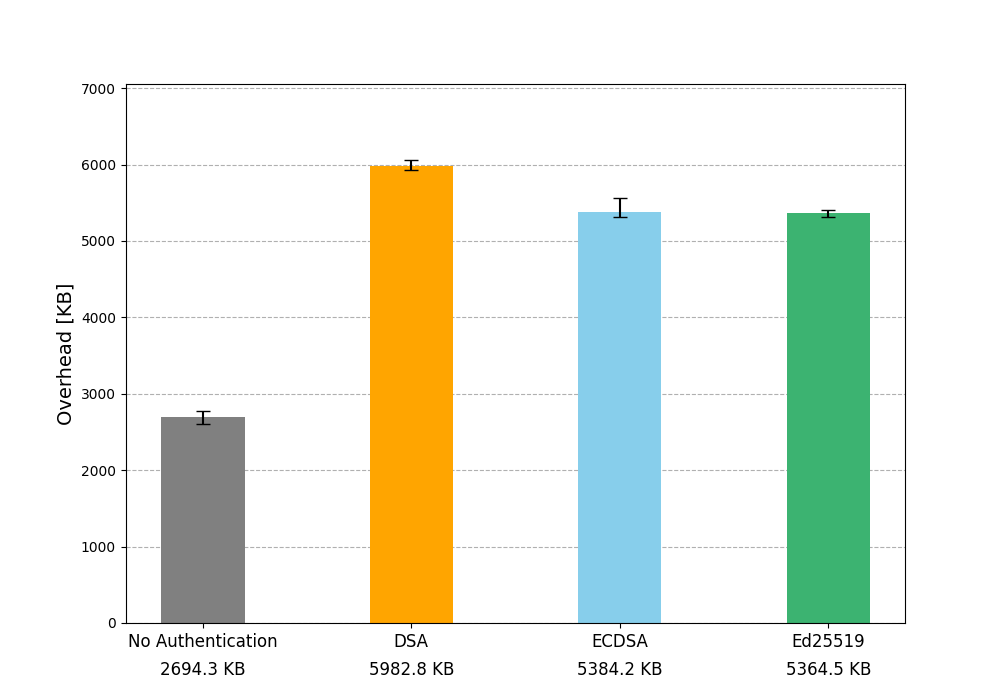
\includegraphics[width=1\textwidth]{figures/exp2_overhead.png}
  \caption{オーバーヘッドサイズ}
  \label{fig:exp2_overhead}
\end{figure}
\FloatBarrier
\indent 図\ref{fig:exp2_delay}は, 実験2におけるシミュレーションパターンごとの
遅延時間を示している. 認証なしでは6.16ms, ECDSAでは5.55ms, EdDSAでは5.31msであった. 
VANETがマルチホップ通信であることから, 選択する経路ごとに遅延が異なり, シミュレーションごとに
ばらつきが生じると考えられる. したがって, それぞれのプロトコルで若干の差異が見られるが, 
3つのプロトコルに特徴的な差が見られないことから, 認証機構の有無は遅延時間に影響を
与えなかったことがわかる. \\
\indent 図\ref{fig:exp2_overhead}は, 実験2におけるシミュレーションパターンごとの
オーバーヘッドサイズを示している. 認証機構なしでは2694.3KBであったのに対し, 
ECDSAでは5384.2KB, EdDSAでは5364.5KBと, 認証機構の追加により
オーバーヘッドサイズが大幅に増加した. これは, Helloパケットの
データに署名が付与されていることが原因である. しかし, EdDSAとECDSAではほとんど差がなかったため, 
署名方式の違いによるネットワークへの負荷は変わらないことがわかる. 
これは, ECDSA と EdDSA の鍵長および署名長が概ね同じ長さであることに起因する結果である. 
なお, 本研究で使用したパラメータによるそれぞれの鍵長は, 
ECDSAとEdDSAともに256ビット, 署名長はECDSAで64バイトから72バイト, EdDSAで64バイトである. \\


